\documentclass{tufte-handout}
\usepackage{listings}
\usepackage{cprotect}
\usepackage{multicol}
\usepackage{graphicx}
\DeclareGraphicsExtensions{.png,.jpg}

\definecolor{dkgreen}{rgb}{0,0.6,0}
\definecolor{gray}{rgb}{0.5,0.5,0.5}
\definecolor{mauve}{rgb}{0.58,0,0.82}

\lstset{language=bash,
  aboveskip=3mm,
  belowskip=3mm,
  showstringspaces=false,
  columns=flexible,
  basicstyle={\small\ttfamily},
  numbers=none,
  numberstyle=\tiny\color{gray},
  keywordstyle=\color{blue},
  commentstyle=\color{dkgreen},
  stringstyle=\color{mauve},
  breaklines=true,
  breakatwhitespace=true,
  tabsize=4,
  upquote=true
}

\title{Git Working!}
\author{SE206 Tutorial}

\begin{document}

\maketitle

\noindent In this tutorial, we'll be covering the basics of git so that you'll be able to use it when working on assignments throughout your degree. We'll be assuming you're on a lab computer running Ubuntu, but if you've gotten git working on a personal device that you are more comfortable with, use that.

\noindent It's recommended that you type out all commands provided rather than copying and pasting them. This is to help you become more familiar with a terminal and get fast at typing stuff out.

\noindent To being with, you're going to want to open up a terminal window and your favourite text editor.

\section{Gitting Started}
\subsection{Initial Setup}

Before we do anything, let's get git setup.

\begin{lstlisting}
$ git config --global user.username "Your Name"
$ git config --global user.email "your_email@example.com"
\end{lstlisting}

\subsection{First Steps}

First, you're going to want to move into your workspace. Then, create a new directory for the repo. Finally, initialise the git repository.

\begin{lstlisting}
$ cd ~/workspace
$ mkdir git-tutorial
$ cd git-tutorial
$ git init # Initalise the directory as a git repo
$ git status # Check the status of the repo
\end{lstlisting}

\noindent Note down what's changed in the directory, what does git status show?

\subsection{Making History}
We'll need to make something into the repo for it to be useful at all. Make anything you want really, but here's something\cprotect\footnote{
	\begin{lstlisting}[language=Python]
	#! /usr/bin/env python

	print 'Hello, world!'
	\end{lstlisting}
}.
Add the file(s) you created to the repo and save it's state with a commit. It's a good idea to check the state of the repo along the way.

\begin{lstlisting}
$ touch hello_world.py # Create a file called hello_world.py
$ vim hello_world.py # Use your favourite editor here.
$ python hello_world.py
Hello, world!
$ git status
$ git add . # Add all files to the repo for tracking
$ git status
$ git commit -m 'hello world' # Save the state of the repo.
$ git status
\end{lstlisting}

\noindent What's printed out by git status? What is an untracked file? Do you know what the . is when adding files? What does the -m option of git commit do?

\section{Branching Out}
\noindent It's time to add an `experimental' feature to our code. We don't want to break master if we make a mistake so we'll be working on a different  branch.

\subsection{Creating a Branch}

\noindent Let's create a branch for experimenting on. We'll call it develop as this is the industry standard.

\begin{lstlisting}
$ git branch develop # Create the new branch
$ git branch # List the branches in the repo
$ git checkout develop # Checkout the newly created branch
$ git status
\end{lstlisting}

\noindent Notice what the current branch is from the output of git branch. Can
you tell what branch you're on using git status?

\subsection{More Changes}

\noindent Time to add that `experimental' feature. Go ahead and change the code to produce something different\cprotect\footnote{
	\begin{lstlisting}[language=Python]
	#! /usr/bin/env python

	print 'Hello, world'
	print 'Hello, Nasser!'
	\end{lstlisting}
}.

\begin{lstlisting}
$ vim hello_world.py
$ python hello_world.py
Hello, world!
Hello, Nasser!
$ git status
$ git diff # See what's changed from the last commit
$ git commit -am 'experimenting'
$ git status
\end{lstlisting}

\noindent What was shown by git diff? Do you understand what it means?

\subsection{Checking the Log}

\noindent Time to review what we've done to the repo. This is achieved by having a look at the log that git keeps automatically.

\begin{lstlisting}
$ git log
\end{lstlisting}

\subsection{Merging changes}
\noindent Everything seems to be working fine so we haven't broken anything. Let's merge the changes we made back into the master branch.

\begin{lstlisting}
$ git checkout master # Move back to the master branch.
$ git log # Display a log of commits in the repo.
$ python hello_world.py
Hello, world!
$ git merge develop # Merge changes from develop into master.
$ python hello_world.py
Hello, world!
Hello, Nasser!
$ git log
\end{lstlisting}

\noindent Notice how after you checkout the master branch, changes you made in the develop branch aren't there until you merge. What does Fast-forward mean in the output of git merge?

\section{Github}

\noindent Time to get your code online! We're going to set up a remote repository and push your changes up to it.

\noindent Head on over to \url{https://github.com} and create an account if you don't have one already. This should be straight forward, but if you have any issues ask a tutor.

\noindent For image guides on how to navigate Github, please see the appendix.

\pagebreak

\subsection{Creating an SSH Key}

\noindent To communicate with GitHub you can either use HTTPS or SSH. HTTPS requires no setup but you will need to enter your username and password every time to make a request to GitHub. SSH on the otherhand uses a public-private key pair to authenticate automatically, however you need to provide GitHub with your public key. We're not going to get into cryptography here, just cover setting it up.

\begin{lstlisting}
$ # Press enter whenever prompted to use the defaults.
$ ssh-keygen -t rsa -C "{YOUR_EMAIL}"
Generating public/private rsa key pair.
Enter file in which to save the key (/{HOME_DIR_PATH}/.ssh/id_rsa):
Enter passphrase (empty for no passphrase):
Enter same passphrase again:
Your identification has been saved in /{HOME_DIR_PATH}/.ssh/id_rsa.
Your public key has been saved in /{HOME_DIR_PATH}/.ssh/id_rsa.pub.
The key fingerprint is:
SHA256:ZkDND3fcLvGgz6eVozHWsbZlPZxwtQHDIwUnSVponFE {YOUR_EMAIL}
The key's randomart image is:
{OMITTED}
\end{lstlisting}

\noindent Now you'll need to copy the public key that was generated and saved in \lstinline!/{HOME_DIR_PATH}/.ssh/id_rsa.pub!. Open the file and copy the contents.

\noindent Head to GitHub and navigate to personal settings. On the left will ``SSH Keys'', click on that. Click ``Add SSH key''. Give the key a title and paste in the key. Click ``Add key''.

\noindent You'll now be able to pull and push to GitHub from the terminal without entering credentials.

\subsection{Creating a Remote Repo}

\noindent First, we need to create a remote repo on github to store a copy of our repo in. You'll need to come up with a cool name for the repo or just use git-tutorial, either will do.

\noindent Github will provide instructions on how to get your code up there, but we'll still cover it here.

\noindent I'll be using \url{https://github.com/drpotato/git-tutorial} as the remote repo in the example.

\begin{lstlisting}
$ # Add a link a remote repository to the local one.
$ git remote add origin git@github.com:drpotato/git-tutorial.git
$ git push --set-upstream --all # Push changes to the remote repo.
\end{lstlisting}

\noindent What do the --set-upstream and --all flags for git push do?

\subsection{Forking}
\noindent Pick a friend or random stranger (or use Chris' repo 
\url{https://github.com/drpotato/git-tutorial}) and fork their repository.

\noindent Once forked, go up a directory and clone your new repo and make some changes \cprotect\footnote{
	\begin{lstlisting}[language=Python]
	#! /usr/bin/env python

	print 'Hello, world'
	print 'Hello, Github!'
	\end{lstlisting}
}.
Be sure to checkout develop, just in case you break the build When you're done, push the changes up to github.

\begin{lstlisting}
$ cd ..
$ # Download a copy of the remote repository
$ git clone git@github.com:drpotato/git-tutorial.git
$ cd git-tutorial
$ git checkout develop # By default it will be on master.
$ vim hello_world.py
$ python hello_world.py
Hello, world!
Hello, Github!
$ git status
$ git diff
$ git commit -am 'changed the hello message'
$ git push origin develop
\end{lstlisting}

\noindent What does git push origin develop do exactly? How is it different from git push --all?

\subsection{Pull Request}

\noindent Now we're going to submit a pull request. This is asking the original repo's owner to go over changes we've made and merge them in if they're acceptable.

\noindent Navigate to your forked github repo on \url{https://github.com}. Click the `Compare, review and create a pull request' button. This will take you to a page to set up a pull request before you fire it off to the owner of the original repo.

\noindent Get your partner to accept your pull request and discuss the changes you made with each other.

\pagebreak
\appendix
\section{Appendix}

Create a repo on Github.

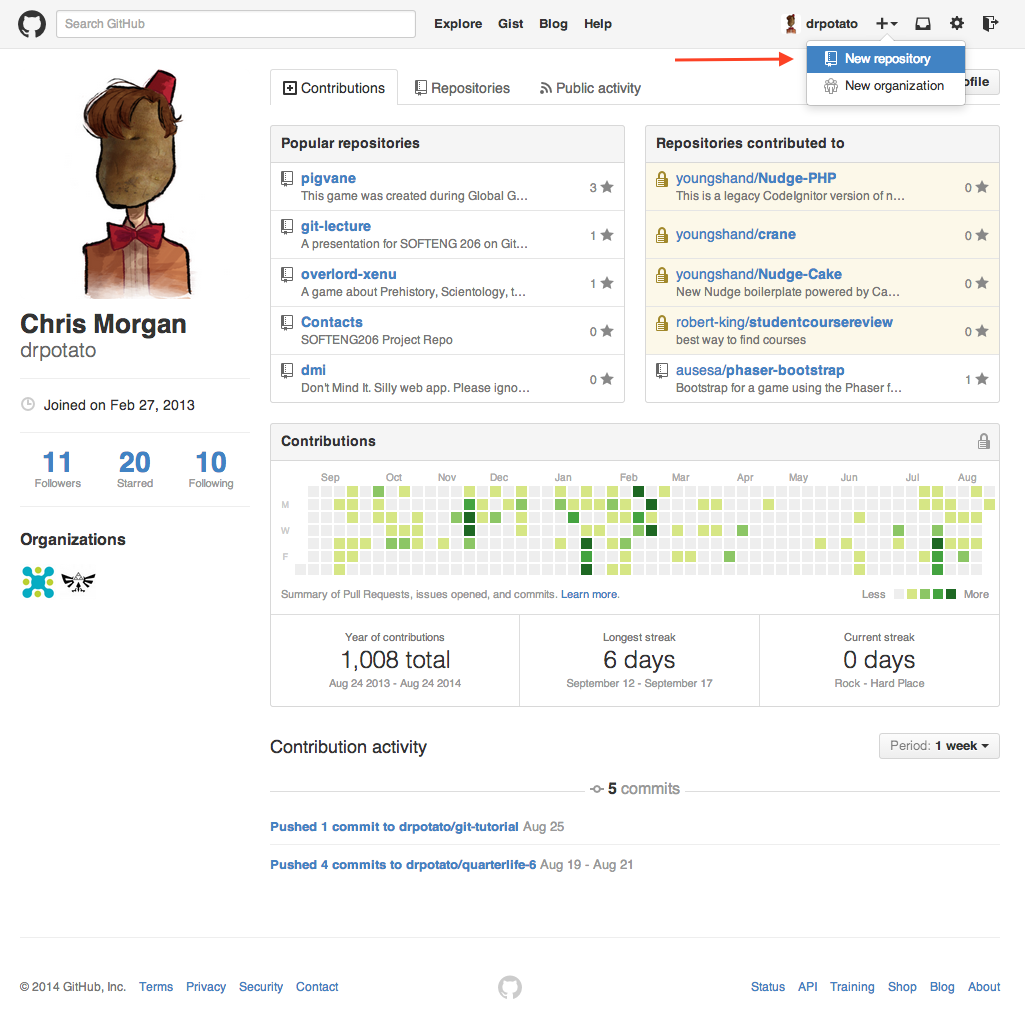
\includegraphics[scale=0.4]{img/github-create-repo.png}

Fork a repo

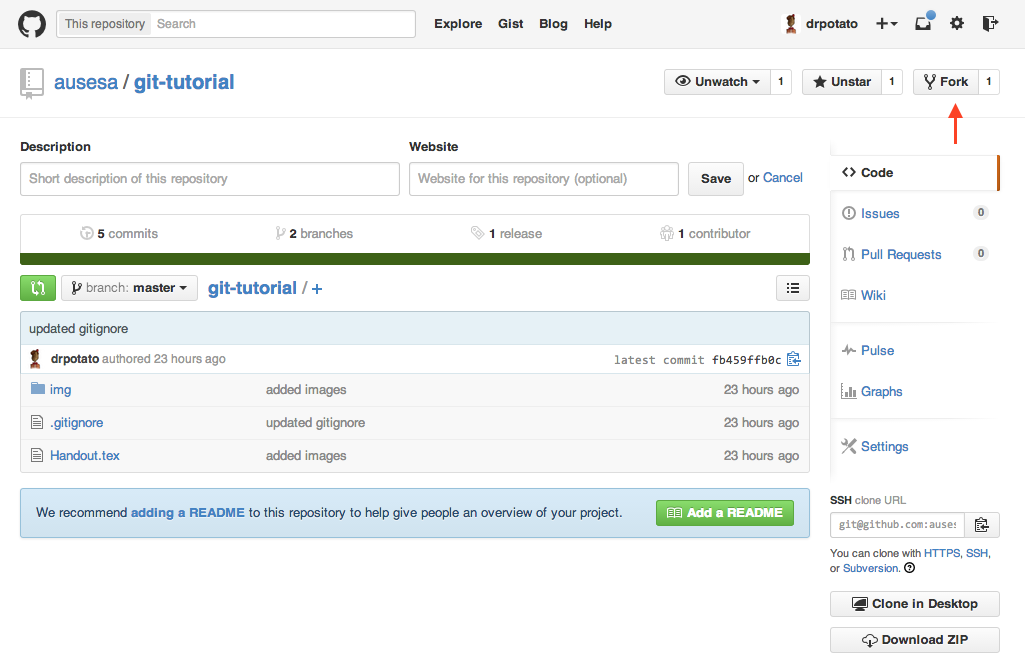
\includegraphics[scale=0.4]{img/github-fork.png}

\pagebreak
Start a pull request.

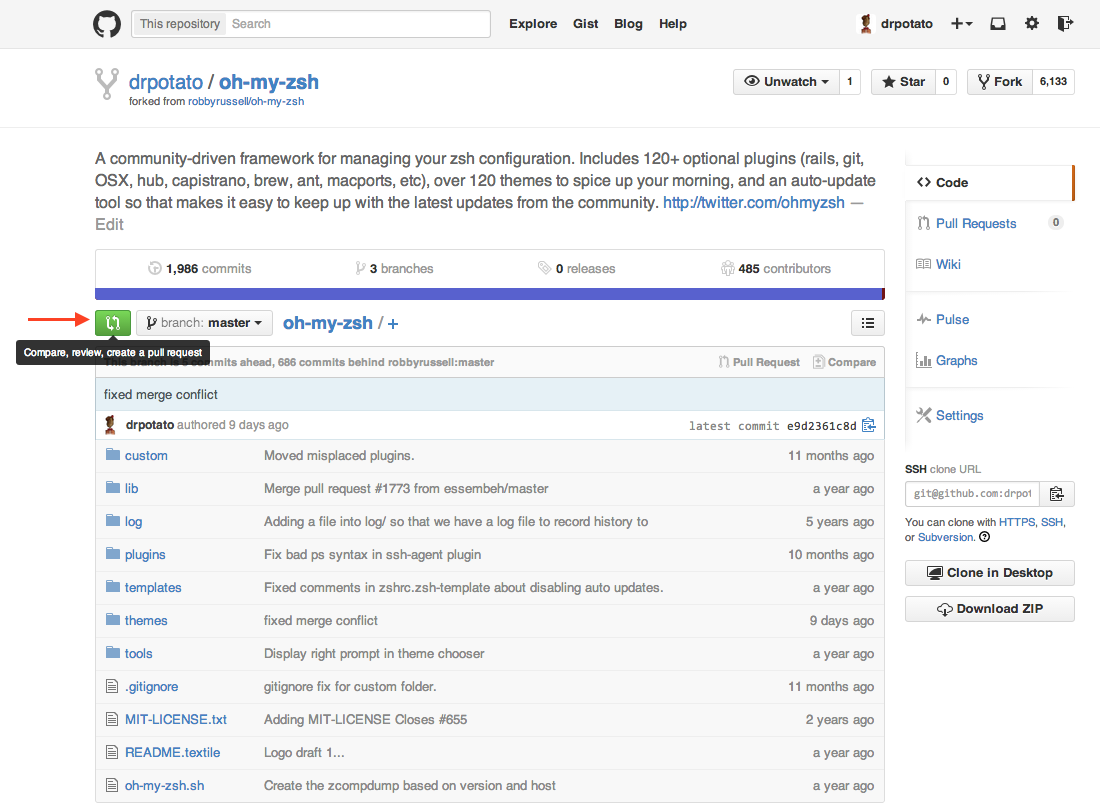
\includegraphics[scale=0.4]{img/github-start-pull-request.png}

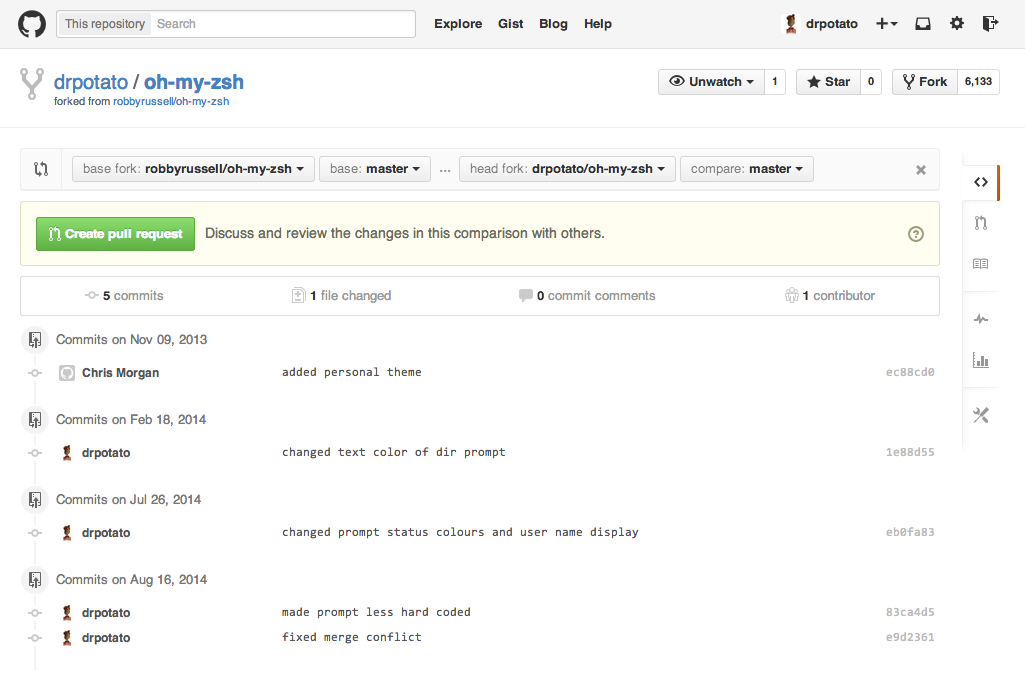
\includegraphics[scale=0.4]{img/github-finish-pull-request.png}

\end{document}